\documentclass[12pt,a4paper]{article}
\usepackage[latin1]{inputenc}			% Encoding
\usepackage{amsmath}
\usepackage{amsfonts}
\usepackage{amssymb}
\usepackage{graphicx}
\usepackage{multirow,multicol}
\usepackage{pifont,hyperref,lastpage,fancyhdr,movie15,float}
\usepackage{eqnarray}
\usepackage{caption}
\usepackage{longtable}
\usepackage{booktabs}
\usepackage{subcaption}
\usepackage[table]{xcolor}
\usepackage{longtable}
\usepackage{booktabs}
\usepackage[total={170mm,257mm}, left=20mm, top=20mm]{geometry}

%%%%%%%%%%%%%%%%%%%%%%%%%%% Footer and Header %%%%%%%%%%%%%%%%%%%%%%%%%%%%%%%%%%%%%%%
\pagestyle{fancy}                                                     				%
\fancyhf{} 		                                                     				%
\lfoot{\tiny\textsf{
\includegraphics[width=1.9cm]{Figures/AIMSCameroonlogo}         %
Po.Box~608 Limbe,~phone~{(+237) 233333363},~                          				%
\url{http://www.aims-cameroon.org}}}                                  				%
\rfoot{\bfseries Page \thepage~of \pageref{LastPage}}                 				%
\renewcommand{\footrulewidth}{2.pt}\renewcommand{\headrulewidth}{0pt} 				%
%%%%%%%%%%%%%%%%%%%%%%%%%%%%%%%%%%%%%%%%%%%%%%%%%%%%%%%%%%%%%%%%%%%%%%%%%%%%%%%%%%%%%

%%%%%%%% Fill here information about the current assignment %%%%%%%%%%%%%%%%%%%%%%%%
\newcommand{\code}{\textbf{IcpO2GR2W1}}                                      %
\newcommand{\deadline}{08.12.24, 11:59 pm}                                         %
\newcommand{\assignment}{assignment [1] ON "Supervised Learning"}				           	   % 
\newcommand{\lecturer}{Lecturer(s): "\textbf{Pr Olawale Awe}"}            		   %
%%%%%%%%%%%%%%%%%%%%%%%%%%%%%%%%%%%%%%%%%%%%%%%%%%%%%%%%%%%%%%%%%%%%%%%%%%%%%%%%%%%%

%%%%%%%%%%%%% Title at the first page %%%%%%%%%%%%%%%%%%%%%%%%%%%%%%%%%%%%%%%%%%%%%%%%%%%
\title{\vspace*{-2cm}\begin{minipage}{\textwidth}                                       %
\begin{center}                                                                          %
\begin{tabular}{|c|c|c|}                                                                %
\hline\multicolumn{3}{|c|}{\bf\scriptsize\MakeUppercase\assignment}\\                   %
\hline{\small Student's Code}&                                                          %
\multirow{3}{7cm}{
\includegraphics[width=7.1cm,height=1.4cm]{Figures/AIMSCameroonlogo}} %
& {\small Deadline}\\                                                                   %
\cline{1-1}\cline{3-3}{\small\bf\code}&&{\small\bf\deadline} \\       					%
\cline{1-1}\cline{3-3}{\small\today} &&{\small Ac. Year: 2024 - 2025}\\           					%
\hline\multicolumn{3}{|r|}{\scriptsize\lecturer}\\\hline              					%
\end{tabular}                                                         					%
\end{center}                                                          					%
\end{minipage}\hfill\date{}\vspace*{-1cm}}                            					%
%%%%%%%%%%%%%%%%%%%%%%%%%%%%%%%%%%%%%%%%%%%%%%%%%%%%%%%%%%%%%%%%%%%%%%%%%%%%%%%%%%%%%%%%%

\newcommand{\K}{\mathbb{K}}
\newcommand{\R}{\mathbb{R}}
\newcommand{\C}{\mathbb{C}}
\newcommand{\D}{\mathbb{D}}
\newcommand{\Z}{\mathbb{Z}}
\newcommand{\N}{\mathbb{N}}

\newtheorem{theo}{Theorem}
\newtheorem{defi}{Definition}
\newenvironment{proof}[1][Proof.]{\textbf{#1~}}{\ \rule{0.5em}{0.5em}}

\begin{document}
\maketitle\thispagestyle{fancy}
\section*{Diagnosing Malaria Using Machine Learning}

\section{Introduction}
Malaria is a life-threatening infectious disease caused by Plasmodium parasites, transmitted to humans through bites of female Anopheles mosquitoes. It primarily manifests as fever, accompanied by symptoms such as chills, headache, nausea, and muscle pain. Factors like poverty, stagnant water, and limited healthcare access exacerbate its spread, leading to complications like anemia, organ failure, or death if untreated. While diagnostic methods like microscopy and rapid antigen tests are available, their reliance on skilled personnel and resources limits their use in low-resource settings.
Machine learning offers a promising alternative by enabling rapid and accurate malaria diagnosis through the analysis of symptoms, clinical data, and diagnostic images. This study explores the application of machine learning for malaria diagnosis, focusing on its potential to enhance accuracy. We begin with a literature review to assess existing methods and advancements in this field, followed by an analysis of machine learning models applied to a malaria dataset. Finally, the discussion highlights the findings, some recommendations, challenges, and future opportunities for leveraging machine learning in combating malaria.

\section{Literature Review}
Machine learning (ML) and data mining techniques have been widely applied to malaria research, emphasizing early diagnosis, treatment optimization, and cost reduction. For instance, studies have shown that ML models outperform traditional statistical methods in predicting malaria outbreaks and diagnosing infections using clinical and demographic data \cite{Li2022}. A systematic review highlights that ML techniques, such as decision trees and random forests, can classify malaria from clinical symptoms and lab results with high accuracy \cite{Zhang2021}. Data mining methods, such as clustering and association rule mining, can process large malaria datasets, revealing hidden patterns that aid in understanding the transmission dynamics. These tools have been used to design diagnostic systems that reduce the risk of misdiagnosis, particularly in areas with limited healthcare access. Ensemble models, which combine various data mining techniques, have been shown to improve predictive accuracy for malaria outbreak forecasting and identifying high-risk areas. Moreover, ML applications have supported drug development by analyzing vast datasets of genetic, clinical, and environmental factors associated with malaria resistance. These advancements have led to more efficient allocation of resources for malaria control and prevention.


\section{Data}

We use on this study a data set call "Malaria-Data.csv" to perform our computation and analysis. \\
This data set contains 18 variables that describe characteristics of the malaria on a patient



	
	\begin{longtable}{lll}
		\caption{variables in the dataset used} \\
		\toprule
		\textbf{Variable Name} & \textbf{Type} & \textbf{Explanation} \\ 
		\midrule
		\endfirsthead
		
		\toprule
		\textbf{Variable Name} & \textbf{Type} & \textbf{Explanation} \\ 
		\midrule
		\endhead
		
		\midrule
		\multicolumn{3}{r}{Continued on the next page...} \\
		\midrule
		\endfoot
		
		\bottomrule
		\endlastfoot
		
		age & Numerical & the age of the patient \\
		sex & categorical &  male or female encoded  with (1,0)\\
		fever & categorical & if yes or no the person has fever \\
		cold & categorical & if yes or no the person is cold \\
		rigor & categorical & if yes or no the person has fever \\
		fatigue & categorical & if yes or no the person is feel tired \\
		headace & categorical & if yes or no the person has headace \\
		bitter tongue & categorical & if yes or no the person has bitter tongue \\
		vomitting & categorical & if yes or no the person vomit \\
		diarrhea & categorical & if yes or no the person has diarrhea \\
		convulsion & categorical & if yes or no the person has convulsion \\
		Anemia & categorical & if yes or no the person has anemia \\
		jundice & categorical & if yes or no the person has jundice \\
		cocacola urine & categorical & if yes or no the person has fever \\
		hypoglycemia & categorical & if yes or no the person has hypoglycemia \\
		prostraction & categorical & if yes or no the person has prostraction \\
		hyperpyrexia & categorical & if yes or no the person has hyperpyrexia \\
		severe maleria & categorical & if yes or no the patient has severe malaria \\
		
		
	\end{longtable}


\subsection{prepossessing}
we used all over our analysis the language R. We started by load the data set and make some prepossessing verification. We check for the type of each column check for missing values and also duplicated value.
\begin{figure}[H]
	\centering
	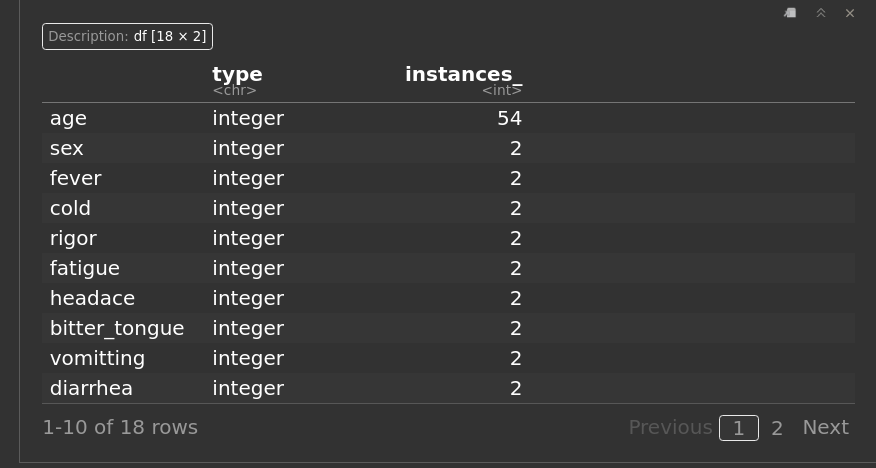
\includegraphics[width=0.9\textwidth, height=0.28\textheight]{Figures/dataType.png}
	\captionof{figure}{variable type and number of distinct value}
	\label{fig:code}
\end{figure}

\begin{figure}[H]
	\centering
	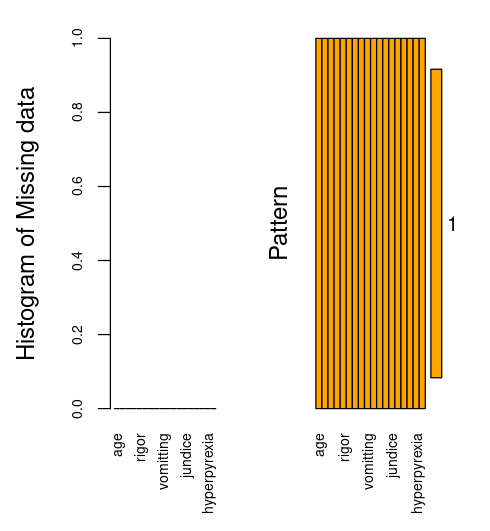
\includegraphics[width=.9\textwidth, height=0.30\textheight]{Figures/missing.png}
	\captionof{figure}{Histogram of missing values}
	\label{fig:code}
\end{figure}

As we can see there where no missing data on the data set which is represented by the pattern fully completed and the histogram of missing value which is empty.\\
\\
After this we where try to check for distributions of both categorical and the numerical variable

	\begin{center}
		\begin{tabular}{ccc} % Three columns
			% First row of images
			\begin{minipage}{0.3\textwidth}
				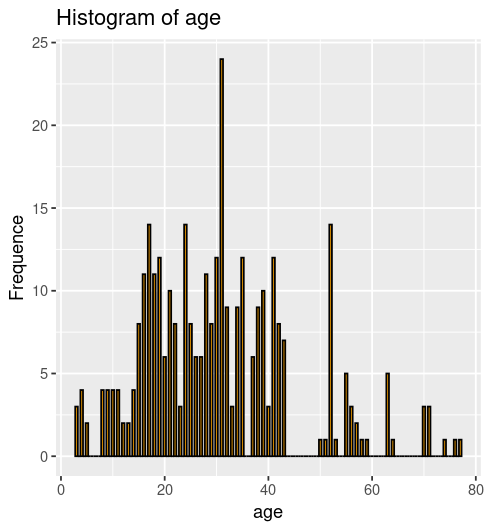
\includegraphics[width=\linewidth]{Figures/Histage.png}
				\captionof{figure}{Histogram age}
			\end{minipage} &
			\begin{minipage}{0.3\textwidth}
				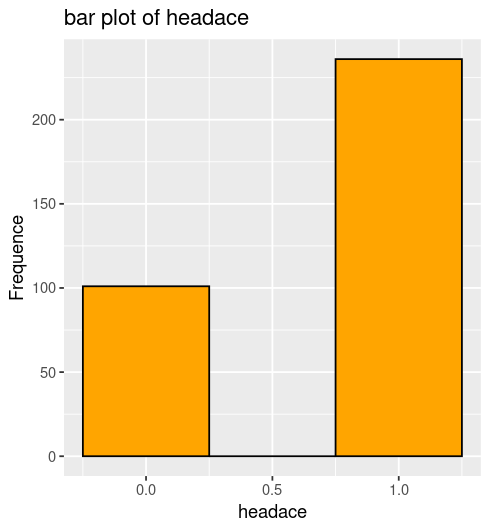
\includegraphics[width=\linewidth]{Figures/BarHeadace.png}
				\captionof{figure}{Bar plot headace}
			\end{minipage} &
			\begin{minipage}{0.3\textwidth}
				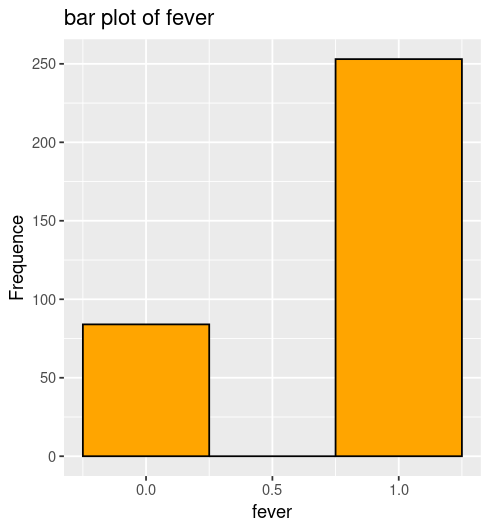
\includegraphics[width=\linewidth]{Figures/BarFever.png}
				\captionof{figure}{Bar plot fever}
			\end{minipage} \\
			
			% Second row of images
			\begin{minipage}{0.3\textwidth}
				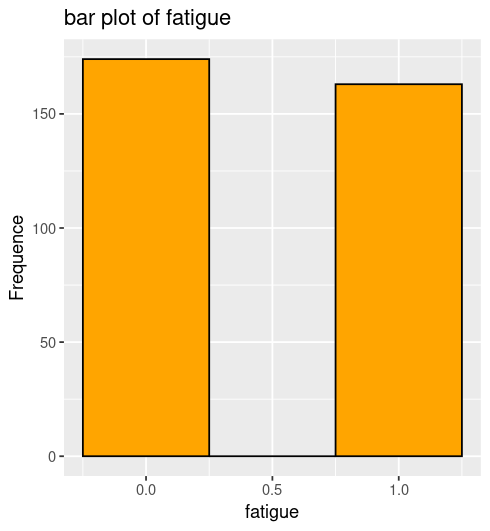
\includegraphics[width=\linewidth]{Figures/BarFatigue.png}
				\captionof{figure}{Bar plot fatigue}
			\end{minipage} &
			\begin{minipage}{0.3\textwidth}
				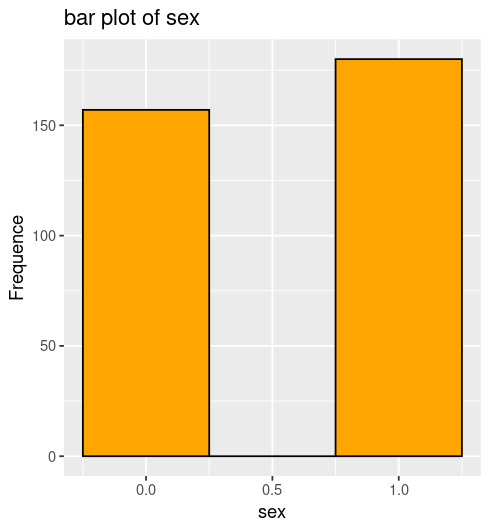
\includegraphics[width=\linewidth]{Figures/BarSex.png}
				\captionof{figure}{Bar plot sex}
			\end{minipage} &
			\begin{minipage}{0.3\textwidth}
				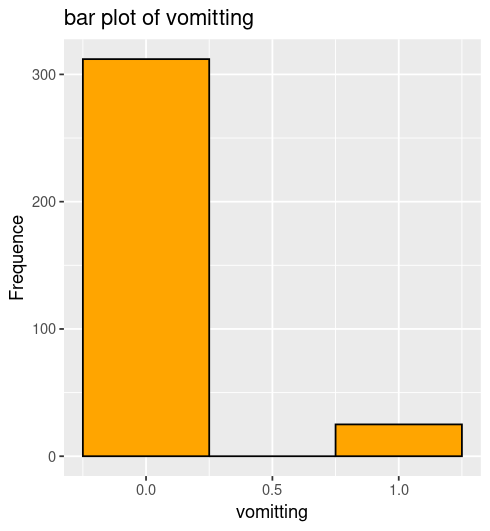
\includegraphics[width=\linewidth]{Figures/BarVomiting.png}
				\captionof{figure}{Bar plot vomiting}
			\end{minipage} \\
		\end{tabular}
	\end{center}

As we can see here:\\ The variable age follow a kind of normal distribution with one outlier who is more old than the other.\\ The observation as imbalance between each of the other variables (there are more tired patient, there are more patient with fever ...)\\ 
In the severe malaria variable which is our target variable which we can observe here,

\begin{figure}[H]
	\centering
	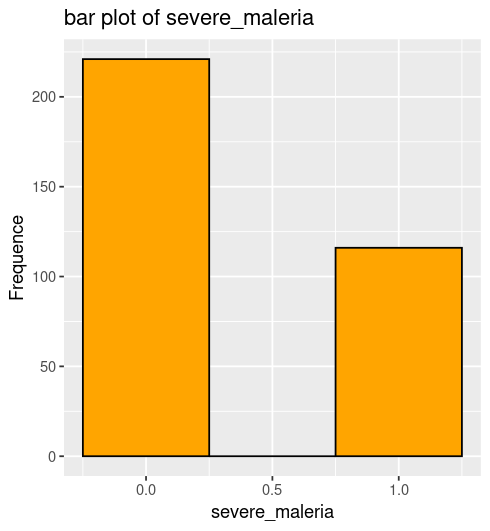
\includegraphics[width=0.4\textwidth, height=0.28\textheight]{Figures/BarSevereMalaria.png}
	\captionof{figure}{Bar plot severe malaria}
	\label{fig:code}
\end{figure}

we see that observation are unequally distributed over the different class 0 (none severe malaria) and 1(severe malaria) so we have here an \textbf{Imbalance data set.}\\
After this we split our data set into two part of 70\% for train and 30% for test
\begin{figure}[H]
	\centering
	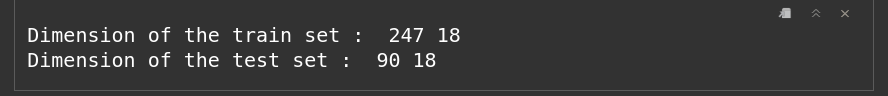
\includegraphics[width=0.9\textwidth, height=0.07\textheight]{Figures/dataspliting.png}
	\captionof{figure}{spliting data}
	\label{fig:code}
\end{figure}

\subsection{Feature Selection}
To perform our analysis we run some variable analysis to see which are the significant variables.\\
we start by running a corelation matrix to see how much variable are correlated and how much and kind of effect each of them has on our target variable.\\
As we can see in the following figure,  all the variable are either almost zero correlated or zero correlated to the severe malaria variable. by this we can not see which variable are important for the model. So we will run another test
\begin{figure}[H]
	\centering
	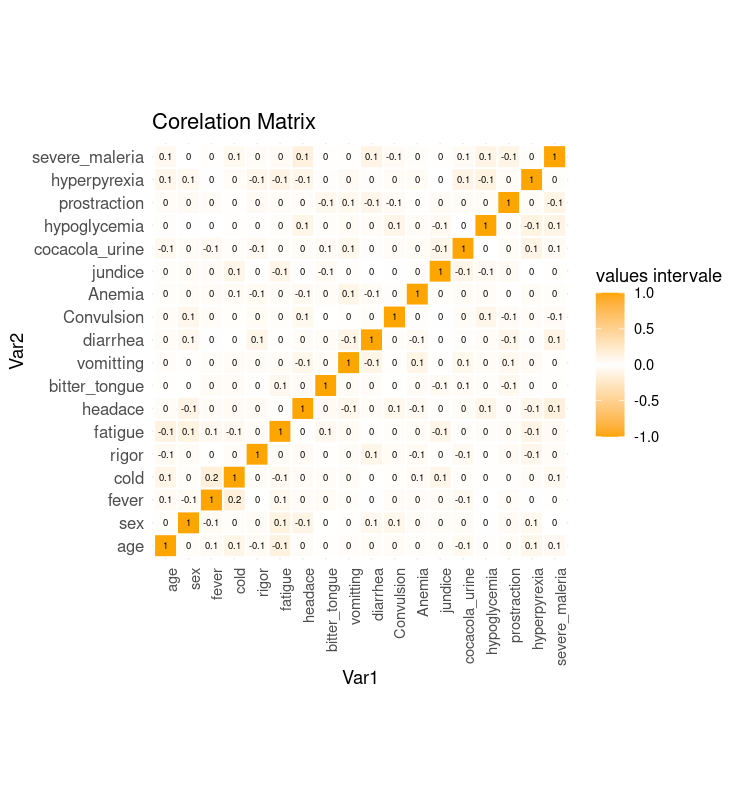
\includegraphics[width=1\textwidth, height=0.6\textheight]{Figures/corMatrix.png}
	\captionof{figure}{correlation matrix data}
	\label{fig:code}
\end{figure}
We have also run a importance variable plot using random forest model to try to get significant variables to explain our target. it is commonly used in machine learning models like decision trees or random forests to indicate how important each variable is in predicting the target outcome.\\
It suggests that a significant portion of the model's accuracy may depend on a few key variables (age,cold head ace or bitter tongue ...). Variables with low importance could potentially be dropped without significantly impacting performance, simplifying the model but Given the small number of features in the dataset, we will include all the
variables in the models if applicable.
\begin{figure}[H]
	\centering
	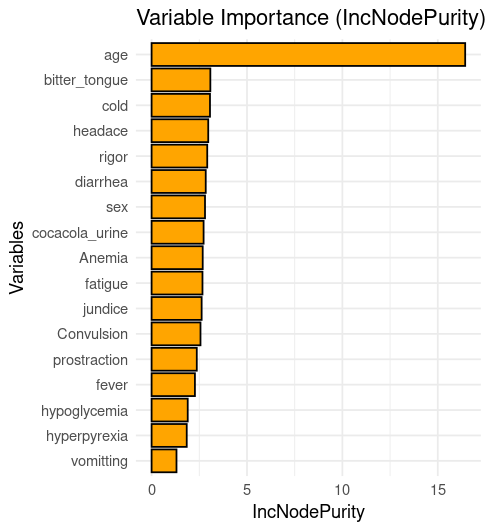
\includegraphics[width=0.5\textwidth, height=0.35\textheight]{Figures/importanceVar.png}
	\captionof{figure}{importance plot}
	\label{fig:code}
\end{figure}


\subsection{Model Training}
After this we run the following model on the imbalance data set 
\begin{longtable}{lll}
	\caption{choosen models} \\
	\toprule
	\textbf{Model Name} \\ 
	\midrule
	\endfirsthead
	
	\toprule
	\textbf{Model Name} \\ 
	\midrule
	\endhead
	
	\midrule
	\multicolumn{3}{r}{Continued on the next page...} \\
	\midrule
	\endfoot
	
	\bottomrule
	\endlastfoot
	
	Logistic Regression \\
	inear Vector Quantization (LVQ) \\
	k-Nearest Neighbors (KNN) \\
	Random Forest \\
	Neural Network \\
	inear Discriminant Analysis (LDA) \\
	Naive Bayes \\
	LightGBM \\
	Support Vector Machine (SVM) \\
	Decision Trees \\
	
	
\end{longtable}

These are all their confusion matrix :
The confusion matrices indicate that the models were tested on imbalanced data, with many struggling to predict the minority class (class 1), as seen in the high red areas for FN and FP. Random Forest (Figure 16) and LightGBM (Figure 20) perform relatively well, with larger green areas in the TP and TN quadrants. Conversely, Naive Bayes (Figure 19) and LDA (Figure 18) show poor performance, marked by significant red in FP and FN. Logistic Regression (Figure 13) struggles with FN errors, making it ineffective for class 1 detection, while SVM (Figure 21) shows moderate performance. Neural Networks (Figure 17) frequently misclassify class 1, while Decision Trees (Figure 22) appear more balanced but prone to overfitting. Models with higher green areas, such as Random Forest and LightGBM, handle imbalanced data more effectively than simpler models like Logistic Regression and KNN.
\begin{center}
	\begin{tabular}{ccc} % Three columns
		% First row of images
		\begin{minipage}{0.3\textwidth}
			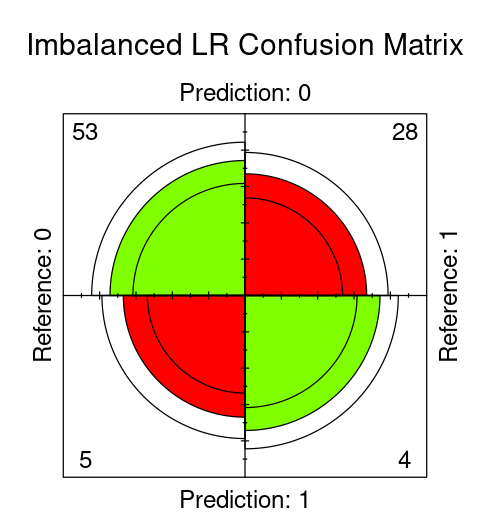
\includegraphics[width=\linewidth]{Figures/IMB_LR.png}
			\captionof{figure}{LR}
		\end{minipage} &
		\begin{minipage}{0.3\textwidth}
			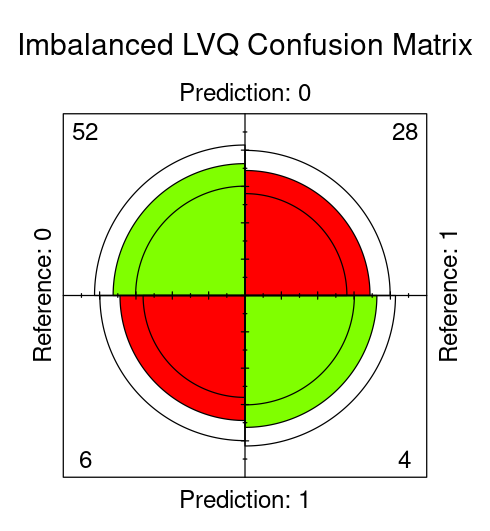
\includegraphics[width=\linewidth]{Figures/IMB_LVQ.png}
			\captionof{figure}{LVQ}
		\end{minipage} &
		\begin{minipage}{0.3\textwidth}
			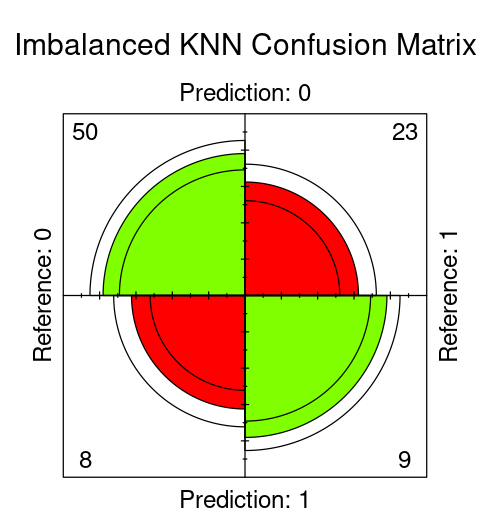
\includegraphics[width=\linewidth]{Figures/IMB_KNN.png}
			\captionof{figure}{KNN}
		\end{minipage}
		 \\
		
		% Second row of images
		\begin{minipage}{0.3\textwidth}
			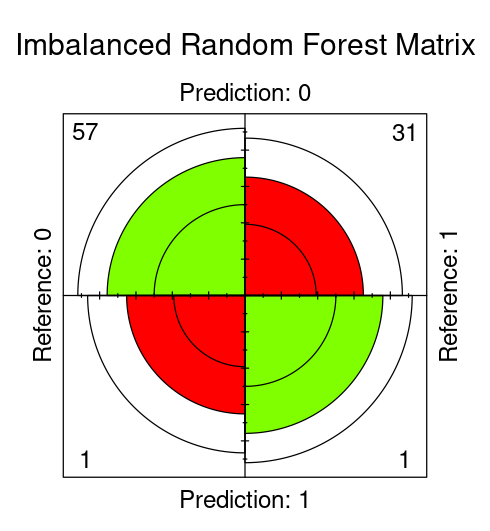
\includegraphics[width=\linewidth]{Figures/IMB_RF.png}
			\captionof{figure}{Random Forest}
		\end{minipage} &
		\begin{minipage}{0.3\textwidth}
			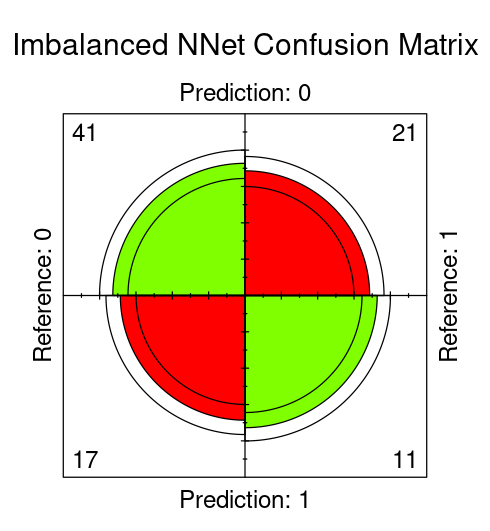
\includegraphics[width=\linewidth]{Figures/IMB_NN.png}
			\captionof{figure}{Neural network}
		\end{minipage} &
		\begin{minipage}{0.3\textwidth}
			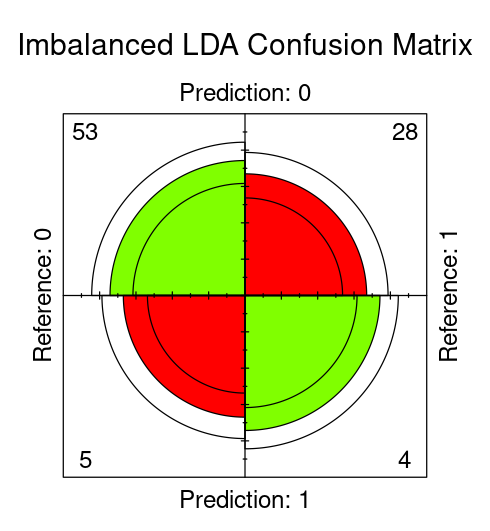
\includegraphics[width=\linewidth]{Figures/IMB_LDA.png}
			\captionof{figure}{LDA}
		\end{minipage} \\
	
		% thirth row of images
		\begin{minipage}{0.3\textwidth}
			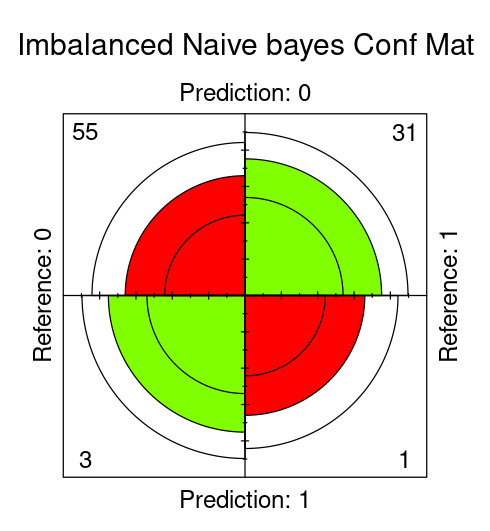
\includegraphics[width=\linewidth]{Figures/IMB_NB.png}
			\captionof{figure}{Naive bayes}
		\end{minipage} &
		\begin{minipage}{0.3\textwidth}
			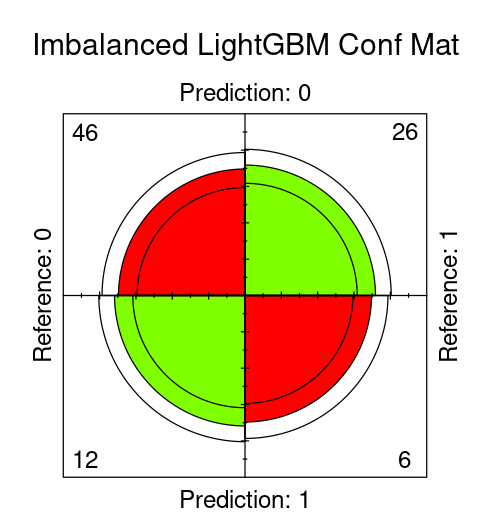
\includegraphics[width=\linewidth]{Figures/IMB_LIGHTGBM.png}
			\captionof{figure}{LightGBM}
		\end{minipage} &
		\begin{minipage}{0.3\textwidth}
			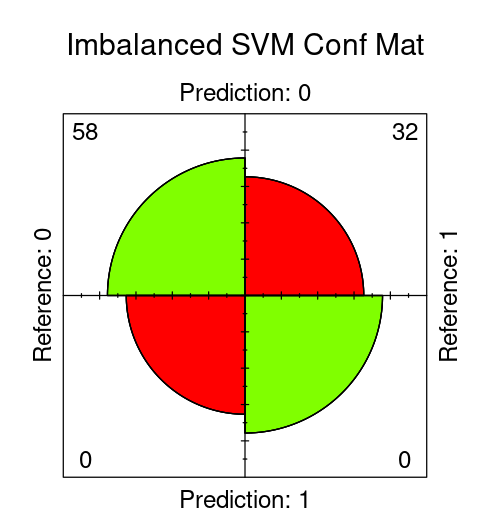
\includegraphics[width=\linewidth]{Figures/IMB_SVM.png}
			\captionof{figure}{SVM}
		\end{minipage} \\
	
		% fourth row of images
		\begin{minipage}{0.3\textwidth}
			
			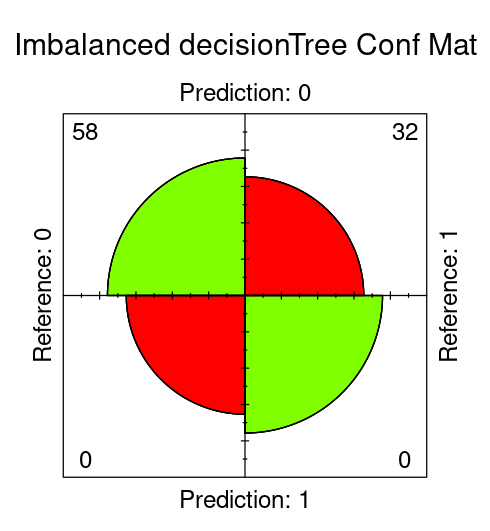
\includegraphics[width=\linewidth]{Figures/IMB_decT.png}
			\captionof{figure}{decision Tree}
		\end{minipage} \\
		\end{tabular}
\end{center}


\subsection{Model Evaluation}
 After running these models on the imbalanced data set we get the following performance metrics which confirm what we were see in the confusion matrix
  \definecolor{lightgreen}{rgb}{0.9,1,0.9}
  \begin{longtable}{llllllll}
  	\caption{Evaluation before oversampling} \\
  	\toprule
  	\textbf{Model} & \textbf{Accuracy} & \textbf{Sensi..} & \textbf{Speci..} & \textbf{b accuracy} & \textbf{precision} & \textbf{f1-score} & \textbf{Mcc} \\ 
  	\midrule
  	\endfirsthead
  	
  	\toprule
  	\textbf{Model} & \textbf{Accuracy} & \textbf{Sensi..} & \textbf{Speci..} & \textbf{b accuracy} & \textbf{precision} & \textbf{f1-score} & \textbf{Mcc} \\ 
  	\midrule
  	\endhead
  	
  	\midrule
  	\multicolumn{8}{r}{Continued on the next page...} \\
  	\midrule
  	\endfoot
  	
  	\bottomrule
  	\endlastfoot
  	
  glm&	0.633	&0.125	&0.9137 &0.519	&0.444	&0.195	&0.061\\	
  lvq&	0.622	&0.125	&0.896 &0.5107	&0.400	&0.190	&0.0328\\	
  rf&	0.644	&0.031	&0.982 &0.507	&0.500	&0.058	&0.045\\	
  \rowcolor{lightgreen}nnet&	0.577	&0.343	&0.706 &0.525	&0.392	&0.366	&0.052\\	
  \rowcolor{lightgreen} lda&	0.633	&0.125	&0.913 &0.519	&0.444	&0.195	&0.0618\\	
  \rowcolor{lightgreen}knn&	0.655	&0.281	&0.862 &0.571	&0.529	&0.3673	&0.175\\	
  nb&	0.622	&0.031	&0.948 &0.489	&0.250	&0.0556	&-0.047\\	
  svm &	0.644	&0.000	&1.000 &0.500	&NaN	&NaN	&NaN\\	
  decision-tree	&0.644	&0.000	&1.000 &0.500	&NaN	&NaN	&NaN\\
  	
  \end{longtable}
  
  \textbf{`In the previous we can see that in term of accuracy:} \\
  The k-Nearest Neighbors (knn) model has the highest accuracy (0.655), suggesting it is \\ better at correctly predicting the outcome overall compared to other models. \\
  
  \textbf{Sensitivity and Specificity:}\\
  Sensitivity (ability to detect positive cases) is highest for the neural network (nnet, 0.343) but very low for models like random forest (rf, 0.031) and naive Bayes (nb, 0.031).
  Specificity (ability to detect negative cases) is perfect for models like SVM and decision tree (1.000), indicating they predict negative cases well but likely fail to identify positive cases due to imbalanced sensitivity.\\
  
  \textbf{Balanced Accuracy:}\\
  Neural network (nnet) has the best balanced accuracy (0.525), showing it balances sensitivity and specificity better compared to others.
  Models like naive Bayes (nb) and random forest (rf) show poor balanced accuracy (~0.50), indicating struggles in handling class imbalance.\\
  
  \textbf{Highlighted LDA Row:}\\
  Linear Discriminant Analysis (lda) has average performance with accuracy (0.633), sensitivity (0.125), and specificity (0.913). However, its F1-score (0.195) and MCC (0.0618) are not strong, suggesting room for improvement in balanced predictions.\\
  
  \textbf{Precision and F1-Score:} \\
  The knn model has the highest F1-score (0.3673), making it effective at balancing precision and recall.
  Models like naive Bayes (nb) and random forest (rf) have very low F1-scores (0.0556 and 0.058), showing poor overall classification performance. \\
  
  \textbf{MCC (Matthews Correlation Coefficient):} \\
  The MCC value for knn (0.175) indicates it has a slightly better correlation between predictions and true outcomes compared to other models. Models like naive Bayes (nb) even have a negative MCC (-0.047), highlighting poor classification performance. \\
  
  \subsection{Evaluation after oversampling}
  \definecolor{lightgreen}{rgb}{0.9,1,0.9}
  \begin{longtable}{llllllll}
  	\caption{Evaluation after oversampling} \\
  	\toprule
  	\textbf{Model} & \textbf{Accuracy} & \textbf{Sensi..} & \textbf{Speci..} & \textbf{b accuracy} & \textbf{precision} & \textbf{f1-score} & \textbf{Mcc} \\ 
  	\midrule
  	\endfirsthead
  	
  	\toprule
  	\textbf{Model} & \textbf{Accuracy} & \textbf{Sensi..} & \textbf{Speci..} & \textbf{b accuracy} & \textbf{precision} & \textbf{f1-score} & \textbf{Mcc} \\ 
  	\midrule
  	\endhead
  	
  	\midrule
  	\multicolumn{8}{r}{Continued on the next page...} \\
  	\midrule
  	\endfoot
  	
  	\bottomrule
  	\endlastfoot
  	
  	glm&	0.655	&0.468 &0.758 &0.613	&0.517	&0.491	&0.232\\	
  	lvq&	0.688	&0.625	&0.724	&0.67	&0.555	&0.588	&0.341\\	
  	\rowcolor{lightgreen}rf&	0.877	&0.750	&0.948		&0.849	&0.888	&0.813	&0.729\\	
  	\rowcolor{lightgreen}nnet&	0.855	&0.906	&0.827 &0.866	&0.743	&0.816	&0.708\\	
  	 lda&	0.666	&0.500	&0.758 &0.629	&0.533	&0.516	&0.2627\\	
  	knn&	0.600	&0.750	&0.517 &0.633	&0.461	&0.571	&0.258\\	
  	nb&	0.555	&0.500	&0.586 &0.5434	&0.400	&0.444	&0.0837\\	
  	\rowcolor{lightgreen}svm &	0.722	&0.593	&0.793 &0.6937	&0.612	&0.603	&0.389\\	
  	decision-tree	& 0.6333 &0.343 &0.793 &0.568	&0.478	&0.400	&0.150\\
  	
  \end{longtable}

	\subsection{Interpretations and recommendation}
	Random Forest (rf) and Neural Network (nnet) are the top-performing models based on the evaluation metrics after oversampling. Random Forest achieves the highest accuracy at 87.7\%, with a balanced accuracy of 84.9\% and a precision of 88.8\%. It also has the highest MCC (0.729), making it a strong choice for handling class imbalances effectively. Neural Network, with an accuracy of 85.5\%, excels in sensitivity (90.6\%) and achieves a competitive F1-score (81.6\%), indicating it detects positive cases well.
	
	SVM performs moderately, with an accuracy of 72.2\% and an MCC of 0.389. However, it doesn't outperform Random Forest or Neural Network in key metrics. Models like Naive Bayes, LDA, and Decision Tree show lower accuracy and MCC values, making them less reliable for this dataset.
	
	Considering all metrics, Random Forest is the recommended model due to its balanced performance, particularly in precision and recall. Neural Network is a strong alternative if sensitivity is the priority. Simpler models like Naive Bayes and LDA are not recommended as they under perform in most metrics.

	\subsection{AUC and ROC}
	
	\begin{center}
	\begin{tabular}{ccc} % Three columns
		% First row of images
		\begin{minipage}{0.3\textwidth}
			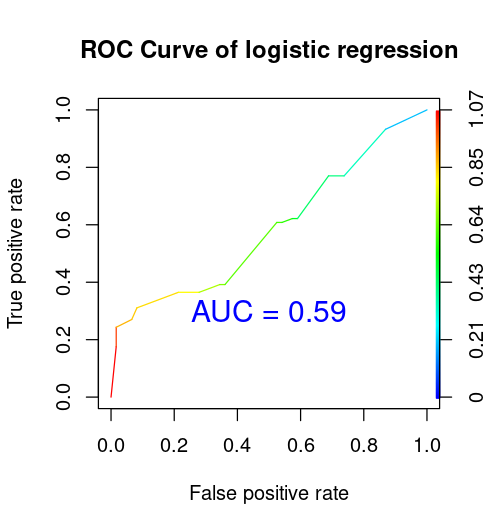
\includegraphics[width=\linewidth]{Figures/AUCLR.png}
			\captionof{figure}{LR}
		\end{minipage} &
		\begin{minipage}{0.3\textwidth}
			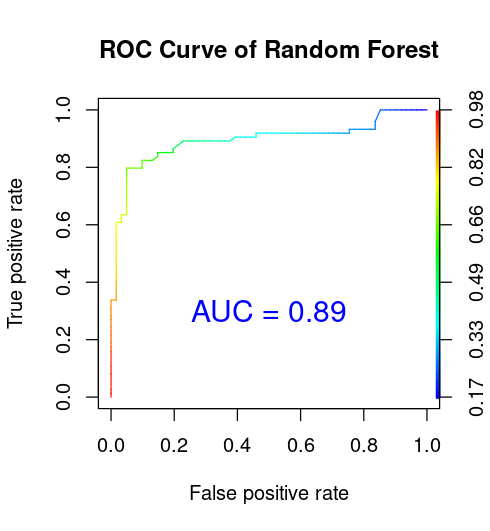
\includegraphics[width=\linewidth]{Figures/AUCRF.png}
			\captionof{figure}{RF}
		\end{minipage} &
		\begin{minipage}{0.3\textwidth}
			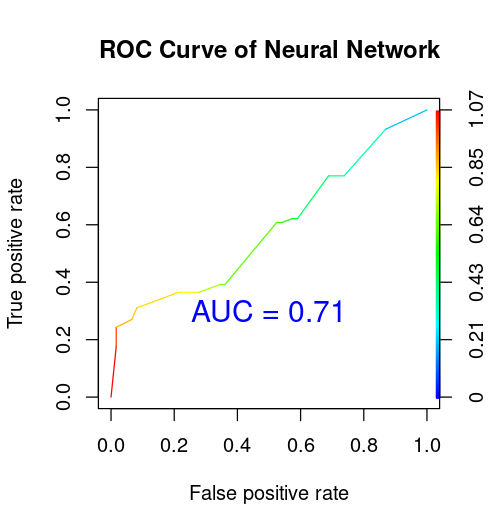
\includegraphics[width=\linewidth]{Figures/AUCNN.png}
			\captionof{figure}{NN}
		\end{minipage}
		\\
		
		% Second row of images
		\begin{minipage}{0.3\textwidth}
			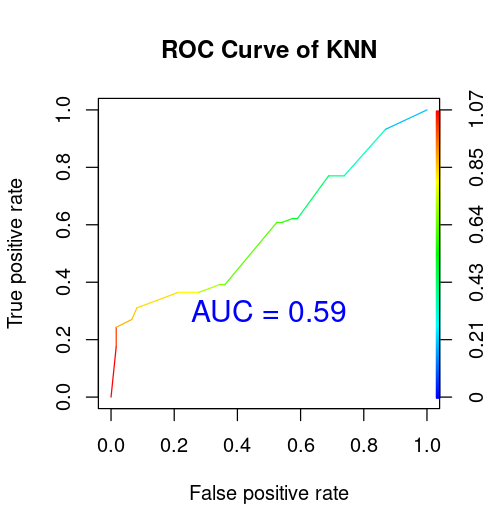
\includegraphics[width=\linewidth]{Figures/AUCKNN.png}
			\captionof{figure}{KNN}
		\end{minipage} &
		\begin{minipage}{0.3\textwidth}
			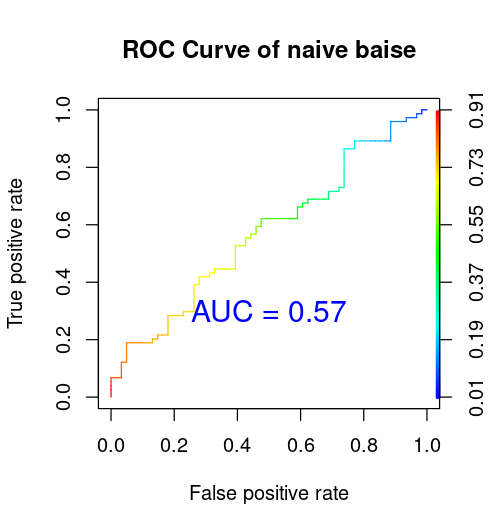
\includegraphics[width=\linewidth]{Figures/AUCNB.png}
			\captionof{figure}{Naive bayes}
		\end{minipage} &
		\begin{minipage}{0.3\textwidth}
			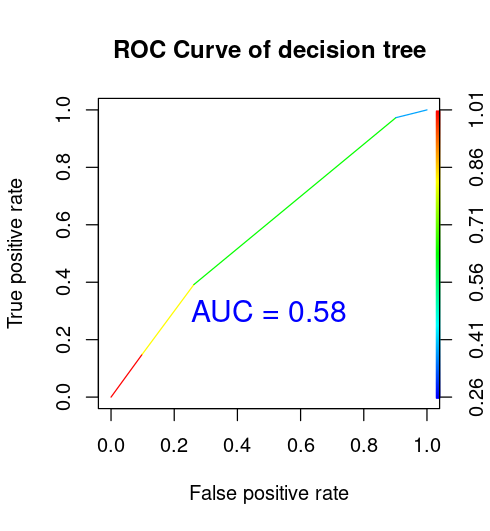
\includegraphics[width=\linewidth]{Figures/AUCDT.png}
			\captionof{figure}{decision Tree}
		\end{minipage} \\
	\end{tabular}
\end{center}

\subsection{Interpretations}
Random Forest (rf) and Neural Network (nnet) are the top-performing models based on the AUC also.

\newpage
\section{Conclusion}
In conclusion, machine learning models (nnet and random forest) offer significant promise for improving malaria diagnosis, especially in low-resource settings and poor significant descriptor. Random Forest outperforms other models with high accuracy, balanced precision, and recall, making it ideal for class imbalances. The Neural Network excels in sensitivity, crucial for detecting positive cases. While SVM, Naive Bayes, LDA, and Decision Trees show moderate performance, they are less reliable for malaria detection. These findings emphasize the potential of machine learning in enhancing diagnostic accuracy and facilitating timely treatment. Further research is needed to optimize these models for real-world use.

















\newpage
\begin{thebibliography}{2}
		
		\bibitem{Li2022} 
		Li, Q., et al., ``Optimizing malaria control strategies using data-driven models: A case study from sub-Saharan Africa,'' \textit{Malaria Journal}, vol. 21, no. 1, p. 25, 2022.
		
		\bibitem{Zhang2021} 
		Zhang, Z., et al., ``Data mining for malaria transmission prediction: A case study using environmental and epidemiological data,'' \textit{Data Science for Health}, vol. 2, no. 1, pp. 50-63, 2021.
	
\end{thebibliography}


\end{document}
